

\title{Erratic-noise suppression using iterative structure-oriented \wen{space-varying} median filtering with sparsity constraint}
\author{Guangtan Huang\footnotemark[1], Min Bai\footnotemark[3], Qiang Zhao\footnotemark[2], Wei Chen\footnotemark[3], and Yangkang Chen\footnotemark[1]}
\renewcommand{\thefootnote}{\fnsymbol{footnote}}
\address{
\footnotemark[1]
School of Earth Sciences\\
Zhejiang University\\
Hangzhou, Zhejiang Province, China, 310027\\
yangkang.chen@zju.edu.cn \\
\footnotemark[2]CNPC Key Laboratory of Geophysical Prospecting\\
China University of Petroleum (East China)\\
Qingdao 266580, China\\
zq\_clark@163.com\\
\footnotemark[3]Key Laboratory of Exploration Technology for Oil and Gas Resources of Ministry of Education\\
Yangtze University\\
Wuhan 430100, China\\
chenwei2014@yangtzeu.edu.cn
}

\DeclareRobustCommand{\dlo}[1]{}
\DeclareRobustCommand{\wen}[1]{#1}

\lefthead{Huang et al., 2020}
\righthead{Erratic noise suppression}

\begin{abstract}
\dlo{Erratic noise refers to those interfering components in the seismic data that correspond to isolated events with the non-Gaussian distribution. Erratic noise is usually of high amplitude, which makes the removal of this type of noise troublesome for many traditional denoising algorithms. We develop a new method to effectively suppress the erratic noise based on an iterative framework. We transform the data \dlo{with}\wen{including} erratic noise to a pseudodata with approximately Gaussian-type noise by \wen{using} a signal-preserving space-varying median filter. The pseudodata can thus be denoised based on a traditional least-squares based method with a sparsity-promoting constraint. Because of the constraint from the space-varying median filtering, strong erratic noise can be effectively suppressed during the iterative procedures. The space-varying filter is applied following the \dlo{morphological pattern of}\wen{slope direction of} the seismic data to further preserve the energy of useful signals. We apply the proposed robust denoising algorithm to a synthetic dataset and two field data examples and find it to be potentially advantageous for a range of industry applications.}Erratic noise often has high amplitudes and a non-Gaussian distribution. Least-squares based approaches therefore are not optimal. This can be handled better with non-least-squares approaches, e.g., based on Huber norm which is computationally expensive.  An alternative method has been published which involves transforming the data with erratic noise to pseudodata that has Gaussian distributed noise. It can then be \dlo{denoised}\wen{attenuated} using traditional least-squares approaches.  This alternative method has previously been used in combination with a curvelet transform in an iterative scheme. In this paper, we introduce a median filtering step in this iterative scheme. The median filter is applied following the slope direction of the seismic data to maximally preserve the energy of useful signals. The new method can suppress stronger erratic noise compared with the previous iterative method, and can better deal with random noise compared with the single-step implementation of the median filter. We apply the proposed robust denoising algorithm to a synthetic dataset and two field data examples and \dlo{find it to be potentially advantageous for a range of industry applications}\wen{demonstrate its advantages over three different noise attenuation algorithms}.   \par
\textbf{Key words:} Seismic signal processing, Erratic noise suppression, Median filtering, Sparsity-promoting constraint
\end{abstract}


\DeclareRobustCommand{\dlo}[1]{}
\DeclareRobustCommand{\wen}[1]{#1}

\section{Introduction}
Strong noise existing in the seismic data often deteriorates many processing and interpretation tasks in the whole seismic imaging workflow, thus the removal of \dlo{the }seismic noise is of great importance \cite[]{liuyang20091,guochang2012,shuwei2016,wangchong2018,zhaoqiang2018}.  According to the difference of spatial correlation in the seismic profiles, seismic noise is usually classified as coherent and incoherent\dlo{ noise}.  Because of the similarity between coherent noise and effective signals in the morphological features, it is usually inadequate to simply apply a one-step filtering method to remove the coherent noise.  Thus, coherent noise, e.g., \dlo{the }ground roll and multiple reflections, is often suppressed via a prediction-and-subtraction strategy \wen{\cite[]{verschuure1991,verschuur1992,karsli2004using,halliday2007,dondurur2012swell,karsli2018mean,zhangdong2020ortho}}. The incoherent noise, however, is mostly suppressed by applying some filters that best utilize the spatially correlative feature of the \dlo{noise}\wen{signal}. %In this paper, we focus on the suppression of incoherent noise.

Suppression of random noise has been studied extensively in recent years. \old{A wide variety of methods}\new{Many methods} have been introduced and applied for \dlo{the }seismic \wen{random-noise} suppression \cite[]{mssa,weilin2016dmssa}. One common \dlo{seismic signal }denoising strategy, \wen{also known as sparse coding}, is to transform the data into different domains in order to concisely represent the signal with a \dlo{few}\wen{limited} number of selected components that capture the useful information \wen{or to further randomize the incoherent components}. \dlo{It}\wen{This strategy} includes \dlo{the }methods based on the Fourier transform \wen{\cite[]{mousavi2016adaptive}}, wavelet transform \cite[]{mostafa2016bssa,mostafa2016geo}, seislet transform \cite[]{fomel2010seislet,yangkang20142}, curvelet transform \cite[]{mostafa2010}, shearlet transform \cite[]{jsedecon2016}, Radon transform \cite[]{beylkin1987discrete}, wavelet transform \cite[]{sweldens1995}, dictionary learning \cite[]{yangkang2017sgk,amir2017,amir2017geo}, and \wen{deep-learning techniques \cite[]{li2018large,zhu2019seismic}}. Another type of approaches for \wen{random-noise attenuation} focus\wen{es} on enhancing useful signals and suppressing random noise by utilizing \dlo{the}\wen{a} predictable property, such as\old{ the} $t-x$ predictive filtering \cite[]{abma1995}, $f-x$ predictive filtering \cite[]{canales1984,gulunay1986},  \new{the} complex-trace analysis method \cite[]{karsli2006application}, non-stationary predictive filtering \cite[]{guochang2012,guochang2013,guochang2018weighted,li2018multidimensional}, and the polynomial fitting-based approach \cite[]{yanhong2009}. \dlo{The decomposition-based denoising approaches consider the disparity of the seismic signal and random noise\wen{,} and attempt to extract useful information from the principal components of the noisy data. Typical methods include the empirical-mode decomposition (EMD) and its improvements ?, singular value decomposition (SVD)-based approaches ?, regularized non-stationary decomposition ?, the Cadzow filtering ?, singular spectrum analysis (SSA) ?, multichannel singular spectrum analysis (MSSA) ?, and damped singular spectrum analysis ?.}

%The decomposition-based denoising approaches consider the disparity of the seismic signal and random noise\wen{,} and attempt to extract useful information from the principal components of the noisy data. Typical methods include the empirical-mode decomposition (EMD) and its improvements \cite[]{chenwei2017emd}, singular value decomposition (SVD)-based approaches \cite[]{yatong2017ieee}, regularized non-stationary decomposition \cite[]{guoning2018}, the Cadzow filtering \cite[]{cadzow1988}, singular spectrum analysis (SSA) \cite[]{ssa,curveletieee2016,amir2017ieee}, multichannel singular spectrum analysis (MSSA) \cite[]{mssa}, and damped singular spectrum analysis \cite[]{weilin2016dmssa}.


Most of the aforementioned denoising algorithms are only effective for Gaussian-type noise. \dlo{The }Gaussian-type noise is usually easy to deal with by a transform-domain thresholding filter based on the least-squares criterion. \old{Erratic noise is also widely seen in many seismic datasets, which, however, is not easy to attenuate using a traditional denoising method.}\new{Erratic noise is also widely seen in many seismic datasets, but is not easy to attenuate using a traditional denoising method.} \dlo{The erratic}\wen{Erratic} noise is often caused by \dlo{a }power line\wen{s}, air blast\wen{s}, cultural noise, polarity reversals, poorly coupled geophones, recording and parity errors, wind, extreme weather conditions, etc \cite[]{trickett2012robust}. The most traditional method to attenuate \dlo{the }erratic noise is by first detecting the abnormal amplitudes and then correcting the amplitudes of the noise positions by interpolation or \dlo{proper }attenuation \cite[]{anderson1989automatic,schonewille2008swell}. A more convenient method is to directly suppress both erratic noise and Gaussian-type noise \dlo{by}\wen{in} a single step. In the past decade, some researchers have realized the necessity in developing algorithms specifically for erratic noise. Some robust denoising algorithms have been developed recently in the literature, such as the robust rank-reduction method \cite[]{chen2014robust} and robust principal component analysis \cite[]{candes2011robust}. The robust rank-reduction method substitutes the least-squares misfit with a more robust misfit function, such as the Tukeys bisquare function \cite[]{beaton1974fitting} or \wen{Huber function \cite[]{huber1964robust,sacchi1997reweighting}}. Both criteria can be connected with \wen{an} L1-norm misfit function to deal with the erratic noise effectively and can be solved with a classic L1 solver. In this way, the robust rank-reduction method is capable of estimating the signals when weakening the influence of \wen{the} erratic noise.  The robust \wen{principal-component} analysis method assumes that the useful signals are of low rank and the erratic noise is sparse. It is possible to construct a convex optimization problem for simultaneously obtaining the low-rank component, i.e., the signal, and the sparse erratic noise. \cite{chen2017robust} further developed an effective method to simultaneously remove erratic and random noise. The estimation of the prediction error filter and the additive noise\old{ sequence} are performed in an alternating fashion. First, the additive noise \old{sequence }is fixed, and the prediction error filter is estimated via the least-squares solution of a system of linear equations. Then, the prediction error filter is fixed, and the additive noise\old{ sequence} is estimated through a cost function containing a hybrid l1/l2-norm that prevents erratic noise to influence the final solution.

\dlo{However, computing}\wen{Computing} these robust criteria requires solving several optimization problems that are highly non-linear \dlo{and}\wen{which} is usually computationally expensive.  \cite{wong2017matrix} theoretically constructed a pseudodata and used the pseudodata to transform a minimization problem with a robust criterion into \dlo{some }well-known minimization problems that can be more easily solved \cite[]{zhaoqiang2018}. This general method has \dlo{a }great potential for transforming a variety of methods into their robust counterparts.  \dlo{Following  ?, we propose a robust version of a traditional sparsity-promoting filtering. To deal with the extremely strong erratic noise, we introduce an extra filtering operator to constrain the pseudodata that helps transform a non-robust minimization problem to a robust one. We apply \dlo{a powerful}\wen{an effective} median filter using a space-varying window size following the morphological pattern of the seismic events to constrain the erratic noise to be in the noise sections.} \wen{Following  \cite{wong2017matrix} and \cite{zhaoqiang2018}, we propose a more effective method to denoise seismic data that contain both erratic and random noise by applying a powerful structure-oriented space-varying median filter \cite[]{sosvmf} \old{into}\new{within} the iterative curvelet thresholding framework \cite[]{zhaoqiang2018}.}

In the proposed algorithm workflow, the \dlo{proposed}\wen{structure-oriented space-varying} median filtering method makes it unnecessary to use a large threshold for the curvelet method and thus makes the whole framework more flexible and reliable. Without the median filtering step, one needs to increase the threshold in the curvelet domain to constrain the erratic noise, thereby removing \dlo{a significant amount of }useful signals. We organize the paper as follows: we first \dlo{introduce}\wen{review} the robust inversion model for noise suppression that we use to suppress both Gaussian-type random noise and erratic noise. \dlo{Then, we introduce in detail a new type of median filter to constrain the pseudodata.}\wen{Then, we review a median filtering technique recently proposed by \cite{sosvmf}. We propose to use this filter to constrain the pseudodata.} Next, we comprehensively analyze the effectiveness and performance of the proposed method over both synthetic and real data examples\dlo{. Finally, some conclusions are made in the end}\wen{, before drawing some conclusions}.
%Some robust denois- ing methods considering erratic noise have been proposed in the past few years, such as robust principal component analysis [56] and robust reduced rank filtering [27], [57]–[61]. The robust principal component analysis supposes that the original data are the superposition of a noisy low-rank signal and a sparse erratic noise. Under this assumption, it is possible to recover both the low-rank and the sparse components exactly from random and erratic noise by solving a very convenient convex problem. Robust reduced rank filtering replaces the sensitive LS criterion by a robust criterion, such as Huber function [62] or Tukeys bisquare function [63]. Those robust criteria combine robust L1-norm treatment of a large erratic noise with Gaussian L2-norm treatment of a random noise [64], and can effectively weaken the influence of erratic noise during denoising. However, this approach suffers from a limitation for real signal in terms of the curve wavefronts that easily violate the low-rank assumption.
\section{Theory}
\wen{\subsection{Robust inversion}
%\subsection{Robust inversion model for noise suppression}
\old{A}\new{An} \wen{$L_1$-norm regularized} least-squares estimate for denoising can be expressed as:
\begin{equation}
\label{eq:ls}
\hat{\mathbf{m}} = \arg \min_{\mathbf{m}} \parallel \mathbf{d} - \mathbf{m} \parallel_2^2 + \gamma \parallel \mathbf{R}(\mathbf{m}) \parallel_1,
\end{equation}
\wen{where $\mathbf{d}$ and $\mathbf{m}$ denote the noisy data and denoised data, respectively, $\mathbf{R}$ is a regularization operator, and $\hat{\mathbf{m}}$ refers to the estimated model.} $\gamma$ is a tradeoff parameter that \dlo{compromise}\wen{compromises} the weight between the data misfit and model constraint.}

\wen{When erratic noise exists, a \dlo{huber}\wen{Huber} norm is better for the denoising problem \wen{\cite[]{wong2017matrix}}:
\begin{equation}
\label{eq:ls2}
\hat{\mathbf{m}} = \arg \min_{\mathbf{m}} \rho_c(\mathbf{d} - \mathbf{m}) + \gamma \parallel \mathbf{R}(\mathbf{m}) \parallel_1,
\end{equation}
where $\rho_c$ denotes the Huber norm. The Huber norm can be expressed as:
\wen{
\begin{equation}
\label{eq:huber}
\rho_c(y) = \left\{\begin{array}{ll}
\frac{1}{2} y^2 & |y|\le c,\\
c(|y|-\frac{1}{2}c) & |y|> c.
\end{array}
\right.
\end{equation}}
The idea of \dlo{constrained }pseudodata is inspired by the robust algorithm proposed in \cite{Oh2007}, where the concept of \emph{theoretical pseudodata} was proposed to transform a \wen{non-linear} optimization problem into a linear least-squares problem. \wen{The pseudodata is a temporary variable during the inversion process, and will be detailed later.} It is \dlo{easy to derive}\wen{easily derived} that, by substituting the raw data $\mathbf{d}$ with the pseudodata $\mathbf{p}$, the subgradient of the objective function with respect to $\mathbf{m}$ in optimization problem \ref{eq:ls} can be expressed as:
\begin{equation}
\label{eq:g1}
g_1=-2(\mathbf{p} - \mathbf{m}) + \gamma \partial_{\mathbf{m}} \parallel \mathbf{R}(\mathbf{m}) \parallel_1,
\end{equation}
where $\partial_{\mathbf{m}}$ denotes the partial derivative with respect to $\mathbf{m}$.}

\wen{Similarly, the subgradient of the objective function in optimization problem \wen{\ref{eq:ls2}} can be expressed as:
\wen{\begin{equation}
\label{eq:g2}
g_2=-\psi_c(\mathbf{d} - \mathbf{m}) + \gamma \partial_{\mathbf{m}} \parallel \mathbf{R}(\mathbf{m}) \parallel_1.
\end{equation}}
\wen{Here, $\psi_c$ denotes the derivative of $\rho_c$.} It is straightforward to derive that \wen{the} two subgradients expressed in \ref{eq:g1} and \ref{eq:g2} are equivalent when:
\wen{\begin{equation}
\label{eq:pseudo0}
\mathbf{p} = \mathbf{m} + \frac{1}{2}\psi_c(\mathbf{d}-\mathbf{m}).
\end{equation}}
}

\wen{$\psi_c$ denotes the derivative of the Huber criterion and can be expressed as:
\begin{equation}
\label{eq:psic}
\psi_c(y) = \left\{\begin{array}{ll}
y & |y|\le c,\\
\text{sign}(y)c &|y|>c.
\end{array}\right.
\end{equation}
\old{The symbol $\mathbf{S}$ denotes a constraining operator to ensure that no erratic noise exists in the pseudodata. In this paper, we propose to use a new type of median filter to filter out the spike-like noise. }The tuning parameter $c$ in equation \ref{eq:psic} can be empirically set as \wen{\cite[]{huber1964robust}}:
\begin{equation}
\label{eq:c}
c=1.345\sigma,
\end{equation}
where $\sigma$ is the approximated standard deviation of the Gaussian-type random noise. Following \cite{holland1977robust}, a robust estimate of $\sigma$ can be chosen as: 
\wen{\begin{equation}
\label{eq:sigma}
\sigma\approx \frac{\text{MAD}}{0.6745} = \frac{\text{Median}|x-\text{Median}(x)|}{0.6745}, 
\end{equation}}
\wen{where MAD denotes median absolute deviation.}}

\wen{\subsection{Iterative curvelet method}
\cite{zhaoqiang2018} proposed to apply the curvelet transform as the regularization operator, i.e., $\mathbf{R}=\mathbf{A}$. $\mathbf{A}$ denotes the curvelet transform. Then the robust inversion model is modified as:
\begin{equation}
\label{eq:ls22}
\hat{\mathbf{m}} = \arg \min_{\mathbf{m}} \rho_c(\mathbf{d} - \mathbf{m}) + \gamma \parallel \mathbf{A}\mathbf{m} \parallel_1.
\end{equation}
Equations \ref{eq:pseudo0} indicates that the minimization of the robust sparsity-promoting denoising model \dlo{equals}\wen{is equivalent} to the case when the input of \wen{a} conventional sparsity-promoting denoising model is a pseudodata expressed in equation \ref{eq:pseudo0}. The pseudodata serves as a bridge to solve a non-linear optimization problem via a linear solver. It is especially advantageous because a number of existing (non-robust) methods can be transformed to their robust counterparts for suppressing erratic noise.}

With $\mathbf{p}$ free of erratic noise, it is possible to use the least-squares model expressed in equation \ref{eq:ls} to remove the Gaussian-type random noise:
\begin{equation}
\label{eq:ls22}
\hat{\mathbf{m}} = \arg \min_{\mathbf{m}} \parallel \mathbf{p} - \mathbf{m} \parallel_2^2 + \gamma \parallel \mathbf{A}\mathbf{m} \parallel_1.
\end{equation}
This denoising problem can be solved simply by a thresholding step:
\begin{equation}
\label{eq:dn}
\hat{\mathbf{m}} = \mathbf{A}^{-1} \mathbf{T}_w \mathbf{A} \mathbf{p},
\end{equation}
where $\mathbf{A}^{-1}$ denotes the inverse sparse transform. $\mathbf{T}_w$ denotes a thresholding operator with an input threshold parameter $w$. The default choice of $w$ is the standard deviation $\sigma$ as approximated in equation \ref{eq:sigma}. In practice, $w$ can be adjusted several times in order to obtain the best performance. It also depends on the \old{sparsity degree}\new{degree of sparsity} in the transform domain. The algorithm formulated as equation \ref{eq:dn} is referred to as the curvelet thresholding method, which will be used in the benchmark comparison in the section of \dlo{EXAMPLES}\wen{examples}. To deal with the erratic noise, equation \ref{eq:ls} is solved iteratively by combining the pseudodata transformation expressed in equation \ref{eq:pseudo0} and the curvelet thresholding method expressed in equation \ref{eq:dn}. This iterative method is referred as the iterative curvelet method \cite[]{zhaoqiang2018}.

\subsection{Structure-oriented space-varying median filter}
Because seismic data is spatially correlative, the traditional median filter needs to be applied in the horizontal dimension of a 2D seismic data for rejecting the spiky erratic noise.  A traditional median filter, however, tends to damage signal energy when the seismic event is dipping. A better way to use the median filter is to apply it along the structural direction of seismic events. To apply the median filter along the structural direction, one needs to extract a 1D vector from the dipping seismic event for the 1D filtering of a median filter. This process is equivalent to flattening the curved seismic events so that the 1D median filter is used easily in the space direction of the flattened gather. 

A critical part in the structure-oriented filtering is the creation of the flattened gather  \wen{in the time-space domain}. %\wen{The flattening process is closely related with the plane-wave destruction operation, which can be expressed briefly as
%\begin{equation}
%  \label{eq:pwd}
%  \mathbf{r} = \mathbf{D(\sigma)\,s},
%\end{equation}
%where $\sigma$ denotes the local slope map, $\mathbf{r}$ is the residual of the plane-wave destruction operation, and $\mathbf{D}$ denotes the plane-wave destruction operator. Equation \ref{eq:pwd} can be formulated as a matrix-vector form:
%\begin{equation}
%  \label{eq:d}
%  \left[\begin{array}{c}
%     \mathbf{r}_1 \\
%     \mathbf{r}_2 \\
%     \mathbf{r}_3 \\
%        \cdots \\
%     \mathbf{r}_N  \\
% \end{array}\right] =
%  \left[\begin{array}{ccccc}
%      \mathbf{I} & 0 & 0 & \cdots & 0 \\
%      - \mathbf{P}_{1,2}(\sigma_1) & \mathbf{I} & 0 & \cdots & 0 \\
%      0 & - \mathbf{P}_{2,3}(\sigma_2) & \mathbf{I} & \cdots & 0 \\
%      \cdots & \cdots & \cdots & \cdots & \cdots \\
%      0 & 0 & \cdots & - \mathbf{P}_{N-1,N}(\sigma_{N-1}) & \mathbf{I} \\
%    \end{array}\right]
%  \left[\begin{array}{c}
%     \mathbf{s}_1 \\
%     \mathbf{s}_2 \\
%     \mathbf{s}_3 \\
%        \cdots \\
%     \mathbf{s}_N  \\
% \end{array}\right]\;,
%\end{equation}
%where $\mathbf{I}$ is an identity operator, $\sigma_i$ denotes the $i$th local slope corresponding to $i$th trace, $\mathbf{s}_i$ denotes the $i$th seismic trace, and $\mathbf{P}_{i,i+1}(\sigma_i)$ denotes the operator that predicts trace $i+1$ from $i$. Prediction between two neighbor traces are achieved by shifting one of the two traces according to the local slope of seismic events. By minimizing equation \ref{eq:d}, the local slope map $\sigma$ can be obtained.}
%
\wen{We do the flattening via recursive prediction between seismic traces based on the estimated local slope.} Assuming that the flattened gather for filtering has a width of $2N+1$,  an arbitrary trace $\mathbf{x}_i$ can be predicted following the equation:
%the central trace $\mathbf{x}_i$ can be predicted from its $j$th ($j\le N$) right trace $\mathbf{x}_{i+j}$ in such a recursive manner,
\begin{equation}
\label{eq:recur}
\mathbf{x}_i=\mathbf{P}_{i+1,i}\cdots\mathbf{P}_{i+j-1,i+j-2}\mathbf{P}_{i+j,i+j-1}\mathbf{x}_{i+j}. 
\end{equation}
\dlo{where $\mathbf{P}_{i,j}$ is an operator, predicting the $i$th trace from the $j$th trace}\wen{Here, $\mathbf{P}_{i,i+1}(v_i)$ is briefly denoted as $\mathbf{P}_{i,i+1}$, where $v$ denotes the local slope at trace $i$}. A similar way can be used to recursively predict $\mathbf{x}_i$ from its left traces by:
\begin{equation}
\label{eq:recur}
\mathbf{x}_i=\mathbf{P}_{i-1,i}\cdots\mathbf{P}_{i-j+1,i-j+2}\mathbf{P}_{i-j,i-j+1}\mathbf{x}_{i-j}. 
\end{equation}

Figure \ref{fig:demo} demonstrates how to construct a structural gather containing flattened events based on the trace prediction strategy. In this sketch, $N=1$. It is obvious that a curved seismic event can be transformed into a flattened event and then the 1D median filter can be used to effectively reject erratic noise in the flattened domain. More details regarding the flattening can be found in \cite{liuyang2010}.

However, the structure-oriented filtering strategy requires the estimation of \wen{the} local slope of an input seismic profile. The challenge in the structure-oriented processing is that we need to obtain a sufficiently accurate slope field for creating \wen{well-flattened} local gathers \cite[]{sosvmf}. In seismic data with strong noise, especially with erratic noise, an accurate slope is difficult or even impossible to obtain.  When \wen{an} inaccurate local slope is obtained, the flattened gather will still contain curved events, which further results in inevitable damages to signals caused by a 1D median filter. In such \dlo{a }case, \dlo{we propose to apply}\wen{\cite{yangkang2015svmf} proposed to use} a space-varying median filter to attenuate the erratic noise in an approximately flattened gather without damaging the useful signals. The filter length $L$ is spatially variable in a space-varying median filter \cite[]{yangkang2015svmf}:
\wen{\begin{equation}
\label{eq:svmf1}
\hat{v}_{i,j}=\arg \min_{v_{m}\in U_{i,j} }\sum_{l=1}^{L_{i,j}} \Arrowvert v_{m} -v_l \Arrowvert_1,
\end{equation}}
where $\hat{v}_{i,j}$ is the output for position $x_{i,j}$. $U_{i,j}=\{v_1,v_2,\cdots,v_{L_{i,j}}\}$ corresponds to a local window for the 1D median filtering.
The spatially variable filter length $L_{i,j}$ can be adaptively chosen as:
\begin{equation}
\label{eq:svmf3}
L_{i,j}=\left\{\begin{array}{ll}
L+l_1,\quad 0\quad \le |x^L_{i,j}|\le T/2 \\
L+l_2,\quad T/2\quad <|x^L_{i,j}|\le T \\
L-l_3,\quad T \quad \le|x^L_{i,j}| < 2T\\
L-l_4,\quad |x^L_{i,j}| \ge 2T
\end{array}\right.,
\end{equation}
where $x^L_{i,j}$ denotes the initial signal estimate at position $x_{i,j}$, which is obtained by applying a median filter (with constant filter length $L$). $T$ denotes the average absolute value of the initial signal estimate. \wen{The variable filter length can better preserve the dipping signal energy since a larger filter length is more powerful in rejecting spiky noise but will damage more signal energy while a smaller filter length is less powerful but more amplitude-preserving, especially for dipping seismic events. The criteria for selecting the window parameters $l_1=2$, $l_2=0$, $l_3=2$, and $l_4=4$, are exactly the same as introduced in \cite{liuyang2009tvmf}. }\wen{It is worth noting that we iteratively calculate the slope and update the input slope for the structure-oriented filtering during the inversion.}

Figure \ref{fig:hyper,hyper-n,hyper-mf0,hyper-sosvmf0,hyper-mf-n,hyper-sosvmf-n} shows a synthetic test of the \dlo{proposed}\wen{enhanced} median filter on a synthetic dataset with hyperbolic events. 
Figures \ref{fig:hyper} and \ref{fig:hyper-n} show the clean and noisy data. Figure \ref{fig:hyper-mf0} and \ref{fig:hyper-sosvmf0} shows the denoising results using the enhanced median filter proposed in \cite{sosvmf}. Correspondingly, Figures \ref{fig:hyper-mf-n} and \ref{fig:hyper-sosvmf-n} show the removed noise. It is clear that the median filtering method proposed by \cite{sosvmf} obtains a successful preservation of seismic events while removing most of the erratic noise. The above mentioned median filter is referred as the structure-oriented space-varying median filter \cite[]{sosvmf}, which will also be used in the benchmark comparison in the section of \dlo{EXAMPLES}\wen{examples}. 

\wen{\subsection{Robust inversion model with an extra constraining operator}
The pseudodata expressed in \ref{eq:pseudo0} depends on the initial estimates of the signal $\hat{\mathbf{m}}$ and noise $\mathbf{n}$. A better estimate of the signal helps obtain a more plausible estimate of $\mathbf{p}$. We propose to iterate the denoising procedures so that we can get the best estimate of the signal where both erratic and Gaussian-type noise are removed while useful signals \wen{remain} untouched.}

\wen{Thus, to}\dlo{To} solve the non-linear optimization problem expressed in equation \ref{eq:ls2}, we first define a \wen{constrained }pseudodata corresponding to the seismic data $\mathbf{d}$ as:
\wen{\begin{equation}
\label{eq:pseudo}
\mathbf{p} = \mathbf{S}(\hat{\mathbf{m}} + \frac{1}{2}\psi_c(\mathbf{n})),
\end{equation}}
where $\mathbf{n}=\mathbf{d}-\hat{\mathbf{m}}$ denotes the noise that corresponds to the signal estimate $\hat{\mathbf{m}}$. \old{$\mathbf{S}$ denotes a constraining operator.}\new{The symbol $\mathbf{S}$ denotes a constraining operator to ensure that no erratic noise exists in the pseudodata. In this paper, we propose to use structure-oriented space-varying median filter to filter out the spike-like noise. }

\dlo{, while} \dlo{Similarly, the subgradient of the objective function in optimization problem \wen{\ref{eq:ls2}} can be expressed as: $g_2=-\psi_c(\mathbf{d} - \mathbf{m}) + \gamma \partial_{\mathbf{m}} \parallel \mathbf{A}\mathbf{m} \parallel_1$.} \dlo{It is straightforward to derive that \wen{the} two subgradients expressed in \ref{eq:g1} and \ref{eq:g2} are equivalent when: $\mathbf{p} = \mathbf{m} + \frac{1}{2}\psi_c(\mathbf{d}-\mathbf{m})$. }
\dlo{Equations \ref{eq:g1}-\ref{eq:pseudo0} indicate that the minimization of the robust sparsity-promoting denoising model \dlo{equals}\wen{is equivalent} to the case when the input of \wen{a} conventional sparsity-promoting denoising model is a pseudodata expressed in equation \ref{eq:pseudo0}. The pseudodata serves as a bridge to solve a non-linear optimization problem via a linear solver. It is especially advantageous because a number of existing (non-robust) methods can be transformed to their robust counterparts for suppressing erratic noise. }

We follow the general framework of the robust matrix completion method developed in \cite{wong2017matrix}. However, the success of the \dlo{transformation by pseudodata}\wen{pseudodata transformation} depends on the selection of the tuning parameter shown in equation \ref{eq:psic}. The parameter $c$ makes the output value of the function $\psi_c$ restricted to $\text{sign}(x)c$, thus alleviating the influence of the outliers. The choice of $c$ is challenging as a large $c$ results in significant residual outliers (erratic noise) while a small $c$ tends to damage the energy of the useful signals. Thus, $c$ remains as an empirical parameter and may vary significantly in extreme cases. To achieve a better compromise between noise removal and signal preservation, we introduce an extra filter $\mathbf{S}$ to constrain the pseudodata, as expressed in equation \ref{eq:pseudo}. \old{With the constrained pseudodata, we can use a relatively large $c$, so that, increasing the variance estimation of Gaussian-type noise $\sigma$, and then use the constraining filter for removing the residual outliers without harming the useful signals.}\new{With the constrained pseudodata, we can use a relatively large $c$, that is, increasing the variance estimation of Gaussian-type noise $\sigma$ and then using the constraining filter for removing the residual outliers without damaging the useful signals.} \cite{zhaoqiang2018} extended this method to seismic data processing by combining the pseudodata transformation with a curvelet thresholding step. We further improve the iterative curvelet method in \cite{zhaoqiang2018} by applying an effective structure-oriented space-varying median filter\old{, which is introduced in detail in the last subsection,} to constrain the pseudodata. In the new framework, a relatively \old{larger}\new{large} $c$ ensures we preserves all signals and some erratic noise. The erratic noise can then be removed by the amplitude-preserving structure-oriented space-varying median filter. Although some signal damages caused by a relatively smaller $c$ can be retrieved during the later iterations, the mixture problem between the signal and erratic noise remains. \old{If some erratic noise has comparative energy as signals}\new{If the erratic noise has comparative energy as the signal}, then it is not possible to separate them using the simple derivative operator of Huber criterion $\psi_c$. In each iteration, the proposed method is better than the traditional method in separating the useful signals, erratic noise, and random noise, thanks to the amplitude-preserving property of the structure-oriented space-varying median filter, which results \new{in} a much better \old{overal}\new{overall} denoising performance.  Thus, selection of $c$ becomes much more convenient and the proposed algorithm framework is almost data adaptive.  
 
\dlo{With $\mathbf{p}$ free of erratic noise, it is possible to use the least-squares model expressed in equation \ref{eq:ls} to remove the Gaussian-type random noise:
$\hat{\mathbf{m}} = \arg \min_{\mathbf{m}} \parallel \mathbf{p} - \mathbf{m} \parallel_2^2 + \gamma \parallel \mathbf{A}\mathbf{m} \parallel_1.$
This denoising problem can be solved simply by a thresholding step:
$\hat{\mathbf{m}} = \mathbf{A}^{-1} \mathbf{T}_w \mathbf{A} \mathbf{p}$,
where $\mathbf{A}^{-1}$ denotes the inverse sparse transform. $\mathbf{T}_w$ denotes a thresholding operator with an input threshold parameter $w$. The default choice of $w$ is the standard deviation $\sigma$ as approximated in equation \ref{eq:sigma}. In practice, $w$ can be adjusted several times in order to obtain the best performance.} 

\dlo{However, the pseudodata depends on \dlo{an}\wen{the} initial estimates of the signal $\hat{\mathbf{m}}$ and noise $\mathbf{n}$. A better estimate of the signal helps obtain a more plausible estimate of $\mathbf{p}$. We propose to iterate the denoising procedures so that we can get the best estimate of the signal where both erratic and Gaussian-type noise are removed while useful signals \wen{remain} untouched.} 

\begin{algorithm}[htb!]
   \caption{Iterative erratic noise suppression algorithm }
   \textbf{Input:} Noisy data $\mathbf{d}$, a pair of forward and inverse sparse transform $\mathbf{A}$ and $\mathbf{A}^{-1}$, a constraining operator $\mathbf{S}$.
    \begin{algorithmic}[1]
    \State \textbf{Initialize $\mathbf{m}_1$ with zero}: $\mathbf{m}_1=\mathbf{0}$
        \For{$i$ = $1,\cdots,N$}
     \State \textbf{Compute}: $\mathbf{n}=\mathbf{d}-\mathbf{m}_i$
     \State \textbf{Compute}: $\mathbf{p}=\mathbf{m}_i+\frac{1}{2}\psi(\mathbf{n})$
     \State \textbf{Compute}: $\mathbf{p}=\mathbf{S}(\mathbf{p})$
     \State \textbf{Solve}: $\mathbf{m}_{i+1}= \arg \min_{\mathbf{m}} \parallel \mathbf{p} - \mathbf{m} \parallel_2^2 + \gamma \parallel \mathbf{A}\mathbf{m} \parallel_1$
     	\If{$\parallel \mathbf{m}_{i+1} - \mathbf{m}_{i} \parallel<\epsilon$} 
     	\State	\textbf{Exit}
     	\EndIf
     
        \EndFor 
%         \State \textbf{1D inverse FFT}: $\hat{D}(x,t)=\text{IFFT}\left(\hat{D}(x,w)\right)$
\end{algorithmic}
   \textbf{Output:} Denoised result $\mathbf{m}_{i+1}$ and noise $\mathbf{n}=\mathbf{d}-\mathbf{m}$.
\label{alg:alg}
\end{algorithm}
Algorithm \ref{alg:alg} \old{detailed}\new{details} the complete workflow of the proposed method. In algorithm \ref{alg:alg}, $\epsilon$ denotes a convergence criterion. In this paper, we define the following convergence criterion:
\begin{equation}
\label{eq:eps}
\epsilon = C\sigma\sqrt{M},
\end{equation}
where $C$ is a gain factor fixed as 1.15 \cite[]{elad2006} and $M$ denotes the dimension of the noisy data $\mathbf{d}$. \wen{The variance} $\sigma$ is the approximated standard deviation of the Gaussian-type random noise, and can be chosen following equation \ref{eq:sigma}. 

The proposed method is not simply a concatenation between a constraining operator (e.g., to remove the erratic noise) and a common random noise attenuation operator. Note that with the transformation expressed in equation \ref{eq:pseudo}, we can update the pseudodata by the current estimations of the model and rejected noise iteratively. For each update, we reformulate the denoising problem as a L1-norm regularized least-squares optimization problem, which can be solved via a standard denoising method. The key difference between the ``hybrid" method and the presented method is that the pseudodata is updated iteratively, thereby transforming the \wen{Huber}\dlo{huber}-norm regularized denoising model to L2-norm regularized denoising model. This strategy is very similar to that used in the well-known iterative re-weighted least-squares (IRLS) method \cite[]{sacchi1997reweighting}.

\dlo{The proposed framework can also be used to reconstruct missing seismic data. In the case of data reconstruction, problem \ref{eq:ls2} can be modified to:
$\hat{\mathbf{m}} = \arg \min_{\mathbf{m}} \rho_c(\mathbf{d} - \mathbf{M}\mathbf{m}) + \gamma \parallel \mathbf{A}\mathbf{m} \parallel_1$,
where $\mathbf{M}$ denotes the sampling operator. Solving the reconstruction problem follows a similar way as in the case of sole noise suppression. }

\dlo{The extension of the proposed iterative framework to the 3D version is straightforward. Since the 3D curvelet transform has been studied extensively in the literature ?, the main difficulty of the 3D extension comes from  the 3D version of the structure-oriented space-varying median filtering. The 3D structure-oriented space-varying median filtering requires the consideration of local slopes from two space directions (e.g., xline and inline) and a 2D median filter. We limit the algorithm tests and discussions in this paper to 2D problems. The 3D extension of the proposed method is now being investigated. }

\section{Examples}
In this section, a synthetic data with simulated Gaussian-type noise and erratic noise is used to \dlo{systematically }evaluate how effective the proposed method is. We also use a real pre-stack marine dataset to illustrate the performance of the proposed \wen{method} in \dlo{real-world applications}\wen{practice}. First, we need to define the metrics to evaluate the performance to quantitatively measure the denoising quality. We utilize the \dlo{SNR}\wen{signal-to-noise ratio} metric that is widely used in the literature. The definition is given as follows:
\wen{\begin{equation}
\label{eq:snr2}
\text{SNR}=10\log_{10}\frac{\Arrowvert \mathbf{s} \Arrowvert_2}{\Arrowvert \mathbf{n} \Arrowvert_2},
\end{equation}}
where $\mathbf{s}$ is the vectorized signal and $\mathbf{n}$ is the vectorized noise. For denoised data, the difference between the exact solution $\mathbf{s}$ and the estimate $\hat{\mathbf{s}}$ is treated as the ``noise". Secondly, we use the local similarity metric as introduced in \wen{\cite{fomel2007localattr}} to evaluate the denoising performance in a local manner. The local similarity measures the correlation between two signals, in a local way. \dlo{For \wen{a} more detailed introduction, readers are referred to -. }\dlo{A higher}\wen{Higher} local similarity between \wen{the} exact solution and the estimate corresponds to \dlo{a }higher accuracy of the estimate, and vice versa.  We can also use the local similarity metric to evaluate the signal damages by calculating the similarity between denoised data and removed noise. A higher local similarity in this case indicates a higher level of signal leakage. This strategy is especially useful for quantifying the denoising performance of the real seismic data example, since there is no ground truth solution for real seismic data and it is \dlo{impossible}\wen{difficult} to use the SNR metric defined in equation \ref{eq:snr2}.  \wen{Thus, in this paper, we use SNR to measure the effectiveness of the methods when dealing with synthetic data and the local similarity metric when dealing with field data.}

The synthetic example is shown in Figure \ref{fig:l_dc,l_dn}. There are 501 time samples and 50 space samples. The sampling rate is 4 ms. Figure \ref{fig:l_dc} and \ref{fig:l_dn} display the noise-free and noise-corrupted data, respectively. There are four linear events in the data. \dlo{Then noisy}\wen{Then, the noise-free} data is corrupted by both Gaussian-type random noise and erratic noise (with \dlo{obviously }strong amplitude). The SNR for the noisy data is -1.25 dB. Figure \ref{fig:l_d} shows a comparison of four denoised results using four different methods. Figure \ref{fig:l_curv} shows the result from a classic curvelet thresholding method \wen{\cite[]{candes20061}}. Figure \ref{fig:l_sosvmf} shows the result from the single-step median filtering method \wen{\cite[]{sosvmf}}. Figure \ref{fig:l_curvi} displays the result from the curvelet method when applied iteratively \wen{\cite[]{zhaoqiang2018}}. Figure \ref{fig:l_sosvmfi} plots the result from the proposed method. The result from the proposed method (Figure \ref{fig:l_sosvmfi}) is obtained after 8 iterations. The result from the iterative curvelet method (Figure \ref{fig:l_curvi}) is obtained after 4 iterations, since more iterations will make the inversion unstable because of the strong erratic noise. The threshold in the curvelet-related methods \wen{(i.e., curvelet method, iterative curvelet method, and the proposed method)} is set as the default value, which is the standard deviation of $\sigma$ as approximated in equation \ref{eq:sigma}. The window length for the median filtering related methods is 9 points. Comparing the four results in Figure \ref{fig:l_d}, it is clear that both curvelet method and iterative curvelet method fail in removing all the high-amplitude erratic noise since there is still some residual erratic noise (especially in the 10th, 19th, 31st traces). The result from the simple median-filtering method does not contain obvious erratic noise but still contains a significant amount of residual Gaussian-type random noise. The result from the proposed method \dlo{obviously }outperforms all the other three methods. The SNRs of the four results are 7.37 dB for the curvelet method, 5.81 dB for the single-step median filtering method, 8.55 dB for the iterative curvelet method, and 9.61 dB for the proposed iterative method. \old{The SNRs of different dataset is also listed in Table \ref{tbl:table1}.}
%\begin{table}[h]
%\caption{SNRs of different method. Curvelet I means direct curvelet thresholding. SOSVMF means single-step median filtering method. Curvelet II means iterative curvelet thresholding.}
%\begin{center}
%    \begin{tabular}{|c|c|c|c|c|c|} 
%  \hline Noisy  & Curvelet I  & SOSVMF & Curvelet II  & Proposed\\ 
%  \hline -1.25 dB & 7.37 dB  & 5.81 dB  & 8.55 dB &  9.61 dB \\
%      \hline
%   \end{tabular} 
%\end{center}
%\label{tbl:table1}
%\end{table}
Figure \ref{fig:l_d_n} shows a comparison of noise removal for all four methods. The removed noise using \dlo{both curvelet-related methods}\wen{curvelet method and iterative curvelet method both} contain some \dlo{useful}\wen{signal} energy from the first dipping event. The removed noise using the proposed median filtering method is obviously weaker than that of the other three methods, especially around the positions of the four linear events. It is also discernible that there are some damages to the signals around the crossing point of the first two seismic events. The noise removed from the proposed method, however, is as strong as the \dlo{curvelet-related}\wen{curvelet and iterative curvelet} methods but does not \old{contains}\new{contain} any observable signal energy. In order to see the iteratively estimated clean signal during iterations, we plot the estimated signals after 1, 3, 5, and 7 iterations in Figure \ref{fig:l_ds}. From Figure \ref{fig:l_ds}, we can observe that the denoised data is getting cleaner and cleaner\old{, and with the amplitude of the first seismic event stronger and stronger}\new{, and that the ampltiude of the first seismic event is gettting stronger and stronger}. This observation can be confirmed from Figure \ref{fig:l_ns}, where the corresponding noise removals are plotted. From Figures \ref{fig:l_n_1} (after 1 iteration) to \ref{fig:l_n_7} (after 7 iterations), we can see clearly that the signal energy corresponding to the first event is getting weaker and weaker. In Figure \ref{fig:l_n_7}, the loss of useful energy is \dlo{barely seen}\wen{significantly less}.

\dlo{The proposed median filter is insensitive to the input slope map.}\wen{The proposed median filter is insensitive to strong variations in the slope map.} The main computational cost of structure-oriented space-varying median filter comes from calculation of the local slope, trace prediction and local similarity calculation required by space-varying median filter in each flattened local gather \cite[]{sosvmf}. \dlo{All these extra computational steps can be implemented via efficient algorithms based on shaping regularization ?, thus the application of this structure-oriented space-varying median filter is not expensive.} The slopes calculated from the noise-free and the noisy data are plotted in \wen{Figures \ref{fig:l_dip_dc} and \ref{fig:l_dip_dn}.} It is clear that the exact solution of \wen{the} local slope is very smooth and correlates \new{well} with the positions of the four seismic events\old{ very well}. The slope calculated from the noisy data, as shown in Figure \ref{fig:l_dn}, however, is highly oscillating and irregular. However, we use the practical slope calculated from the noisy data for the structure-oriented space-varying median filtering and the performance is still \dlo{successful}\wen{excellent}. It is worth mentioning that if we use a traditional structure-oriented space-varying median filtering method, the performance will highly \dlo{depends}\wen{depend} on the input slope map, which is very inaccurate in this example. We iteratively calculate the slope and update the input slope for the structure-oriented filtering during the inversion. The calculated slopes after 1, 3, 5, and 7 iterations are shown in Figure \ref{fig:l_dips}. From (a) to (b) in Figure \ref{fig:l_dips}, it is clear that the \dlo{slope}\wen{slopes} \dlo{becomes}\wen{become} smoother\dlo{ and smoother} and more accurate \dlo{as}\wen{when} compared with the exact solution in Figure \ref{fig:l_dip_dc}. \dlo{\dlo{But the}\wen{The} slope calculated after \dlo{7}\wen{seven} iterations is much better than the original input slope in Figure \ref{fig:l_dip_dn}, but is still a bit different \dlo{with}\wen{compared to} the exact solution.} We iteratively calculate the SNRs during the inversion and show the SNR diagram in Figure \ref{fig:l_snrs4}. In the first \dlo{6}\wen{six} iterations, the SNR increases from less than 6 dB of the initial estimate to around 10 dB. After \dlo{even}\wen{the} first iteration, the SNR has a dramatic change. After \dlo{6}\wen{six} iterations, however, the SNR goes through a small drop, which is explained by the fact that the proposed iterative \dlo{retrive}\wen{procedure retrieves} useful signals back from the removed noise while also \dlo{getting }\wen{re-introducing }some Gaussian-type noise\dlo{ back}. Although SNR decreases, the overall performance actually keeps increasing, as confirmed from the \dlo{iteratively}\wen{iterative} output results plotted in Figures \ref{fig:l_ds} and \ref{fig:l_ns}.

\wen{In Figure \ref{fig:l_dds}, we show iteratively obtained}\dlo{We also show iteratively obtained} results using the curvelet method, i.e., iteration without applying the proposed median filter as a constraining operator\dlo{, in Figure \ref{fig:l_dds}}. Figures \ref{fig:l_dds}a-\ref{fig:l_dds}d correspond to the output result after 1, 3, 5, and 7 iterations, respectively. From this comparison, we see that in the first 3 iterations, the iterative curvelet method is still stable, \dlo{then}\wen{following this} the iterative method becomes unstable because we iteratively retrieve the high-amplitude erratic noise from the noise profile without constraint to suppress the erratic noise. The corresponding noise profiles are shown in Figure \ref{fig:l_nns}, where we see that the removed noise becomes \dlo{weaker and weaker, indicating the fact that the iteration becomes less and less effective}\wen{weaker, indicating that progressive iterations become less effective}. The SNR comparison can only provide a global evaluation of the denoising performance. We then use the local similarity to evaluate the denoising performance\dlo{ locally}. The local \dlo{similar}\wen{similarity} maps between the noise-free data and the denoised data using different methods are shown in Figure \ref{fig:l_simi}. The high anomalies on the local similarity maps correlate with the seismic events very well. However, the amplitude of the local similarity anomaly is different for the four methods. While all the methods except for the proposed method have similar local similarity, the proposed method obtains \dlo{obviously }higher similarity values. To measure the signal leakages \cite[]{yangkang2015ortho}, the local similarity between the denoised data and removed noise for different methods are then calculated and shown in Figure \ref{fig:l_simi2}. It is clear that both \dlo{curvelet-related}\wen{curvelet and iterative curvelet} methods have some high similarity anomalies along the first seismic event, indicating the signal leakage of the first seismic event. The local similarity of the single-step median filtering method shows \dlo{obvious }high anomalies in the middle part of the profile. It is \dlo{salient}\wen{clear} that the local similarity corresponding to the proposed method is mostly zero and negligible across the whole profile. In order to test the denoising performance of different noise levels, e.g., in terms of random noise intensity and erratic noise density, we further conduct two tests. The first test is to explore the denoising performance of the proposed method in the cases of different noise intensities. We increase the noise variance gradually and apply the proposed method to compare the denoising performance. This test is illustrated in Figure \ref{fig:sigmas_d}. The top row of Figure \ref{fig:sigmas_d} show the noisy data with the same erratic noise but with increasing random noise intensity. The bottom row of Figure \ref{fig:sigmas_d}  shows the \old{correspondingly}\new{corresponding} removed noise sections. It is clear the denoising performance decreases as the noise variance increases. The denoising performance in the case of the strongest random noise is still acceptable, except for relatively more residual noise. Next, we conduct a similar test in terms of different erratic noise densities. This test is illustrated in Figure \ref{fig:dens_d}. The top row of Figure \ref{fig:dens_d} shows the noisy data with the same random noise but with increasing erratic noise density. The bottom row of Figure \ref{fig:dens_d} shows the \old{correspondingly}\new{corresponding} removed noise. It is obvious that the denoising performance decreases as the erratic noise density increases. When the erratic noise is the most dense, there is some residual noise in the result, but the general performance is still acceptable. These two tests show that the proposed method could perform robustly in cases when noise levels are high. 



We further test the proposed method on a real seismic data as shown in Figure \ref{fig:f_dn}. This dataset is a \dlo{marin}\wen{marine} pre-stack shot gather, which contains both Gaussian-type random noise and erratic noise. There are 800 time samples and 220 space samples. The sampling rate is 4 ms. The results from the four aforementioned methods are shown in Figure \ref{fig:f_d}. From Figure \ref{fig:f_d}, it is clear that \dlo{both curvelet-related methods}\wen{both curvelet and iterative curvelet methods} have successfully \dlo{attenuate}\wen{attenuated} the Gaussian-type random noise but fail in \dlo{rejecting}\wen{removing} \dlo{those}\dlo{the}\wen{all} erratic noise. The iterative curvelet method seems to suppress more erratic noise than the simple curvelet thresholding method. The proposed median filter, although \wen{successfully rejecting} all the erratic noise, fails in attenuating much \wen{of} Gaussian-type random noise. The proposed method, as shown in Figure \ref{fig:f_sosvmfi_n}, obtains a very satisfying result with both \wen{the} Gaussian-type random noise and erratic noise effectively removed. In this example, both iteration-related methods use 8 iterations to obtain the result. The given window length for the median filters are both 9 points. A comparison of the removed noise profiles is shown in Figure \ref{fig:f_d_n}. It is obvious that both \dlo{curvelet-related}\wen{curvelet and iterative curvelet} methods tend to cause significant signal leakage.  The median filtering-related methods are very effective in preserving all the useful signals. \wen{However, it seems that the single-step median filtering removes less noise, compared with the proposed method.} Figure \ref{fig:f_ds} shows a comparison of \dlo{iteratively output}\wen{the iterative output} result after 1, 3, 5, and 7 iterations. It is clear that the high-amplitude erratic noise is well constrained during the iterations due to the effectiveness of the proposed median filter, and the amplitude of \wen{the} useful signals \dlo{becomes higher and higher}\wen{becomes progressively higher}. This observation can be further validated from the comparison of removed noise profiles during iterations in Figure \ref{fig:f_ns}. From (a) to (d) in Figure \ref{fig:f_ns}, it is clear that the signal leakage is gradually \dlo{retrieved}\wen{reduced} and the noise profile after 7 iterations \dlo{is almost not containing}\wen{contains almost no} discernable signal energy. In this example, because the exact solution for the noise-free data is unknown, we cannot use the SNR for evaluating the denoising performance. In this case, the local similarity is used to measure the signal damages of \wen{the} different methods. Here, we want to emphasize again that based on a similar level of removed noise, the local similarity can help measure how a method can preserve\dlo{/damage} the useful signals by simply checking the \dlo{high-anomalies}\wen{high-amplitude anomalies} in the similarity maps. The local similarity maps are plotted in Figure \ref{fig:f_simi2}, where we can observe that \dlo{both curvelet-related}\wen{both curvelet and iterative curvelet} methods cause significant signal leakages around the right side of the first arrivals. The single-step median filtering causes some damages in the areas around the first arrival. The proposed method does not cause observable signal leakage, indicating \dlo{a }\dlo{perfect}\wen{a very good} preservation of \wen{the} useful signals. 

Next, we test the proposed method on another real data example, which is a post-stack seismic data. The raw data is plotted in Figure \ref{fig:f2_d}. There are 256 time samples and 256 space samples. The sampling rate is 4 ms. This example contains very strong string-like erratic noise and moderately strong Gaussian-type random noise.  The four results using four different methods are plotted in Figures \ref{fig:f2_curv}-\ref{fig:f2_sosvmfi}. The removed noise sections corresponding to different methods are plotted in Figure \ref{fig:f2_d_n}. The red arrows highlight the differences among the four methods. As emphasized by the red arrows, both \dlo{curvelet-related}\wen{curvelet and iterative curvelet} methods damage significant signal energy while the median filter-related methods preserve the useful signals well. Compared with the single-step filters, the two iterative methods remove more noise. Although the iterative curvelet method seems to be cleaner, \old{however, }it causes significant damages to the useful signals, as highlighted in Figure \ref{fig:f2_curvi}. \wen{It is also observable that the proposed method causes a few sporadic residual spikes. Considering the overall performance, these spikes are negligible.} It is intuitive that noise removal and signal preservation are always a compromise. \old{The traditional median filter is not as competent as the structure-oriented space-varying median filter in compromising the two things.}\new{The structure-oriented space-varying median filter better defines the tradeoff between the two than the traditional median filter.} Besides, the structure-oriented space-varying median filter \cite[]{sosvmf} \old{is more convenient to adapt}\new{more readily adapts} to the complexity of the input seismic data. More importantly, it is used in a data-driven way, i.e., insensitive to the noise levels or structural complexity (as elaborated in \cite{sosvmf}).


\section{Discussions}
\wen{The extension of the proposed iterative framework to the 3D version is straightforward. Since the 3D curvelet transform has been studied extensively in the literature \cite[]{ying20053d,jingjie2015jse}, the main difficulty of the 3D extension comes from  the 3D version of the structure-oriented space-varying median filtering. The 3D structure-oriented space-varying median filtering requires the consideration of local slopes from two space directions (e.g., xline and inline) and a 2D median filter. We limit the algorithm tests and discussions in this paper to 2D problems. The 3D extension of the proposed method is now being investigated. }

The proposed framework can also be used to reconstruct missing seismic data. In the case of data reconstruction, problem \ref{eq:ls2} can be modified to:
\begin{equation}
\label{eq:ls_recon}
\hat{\mathbf{m}} = \arg \min_{\mathbf{m}} \rho_c(\mathbf{d} - \mathbf{M}\mathbf{m}) + \gamma \parallel \mathbf{A}\mathbf{m} \parallel_1,
\end{equation} 
where $\mathbf{M}$ denotes the sampling operator. Solving the reconstruction problem follows a similar \old{way as in the case of sole noise suppression}\new{approach as the noise suppression problem}.

The proposed framework is more capable of compromising \new{between} the removal of erratic and random noise, and preservation of signal energy, thanks to the \old{superb amplitude-preserving  performance}\new{amplitude preservation} offerred by the structure-oriented space-varying median filtering. \old{The amplitude preserving property enables the proposed method useful for the amplitude-variation-with-offset analysis.}

\section{Conclusions}|


Most traditional denoising methods designed for Gaussian-type random noise may fail if the seismic data is also corrupted by erratic noise. To resolve this problem, in this paper, we combine the methods of \cite{wong2017matrix}, \cite{zhaoqiang2018} and \cite{sosvmf}. The general idea of pseudo-data transformation was from \cite{wong2017matrix}. Then, \cite{zhaoqiang2018} improved \cite{wong2017matrix}'s method by introducing the curvelet method. Next, we further improve \cite{zhaoqiang2018}'s method by introducing \old{a more }\new{an} advanced median filtering method \new{\cite[]{sosvmf}} to better cope with the structural complexity. On the other hand, the proposed method in this paper improves the structure-oriented space-varying median filtering method \cite[]{sosvmf} by better coping with the random noise. The proposed approach is tested on a synthetic and two real seismic data containing strong erratic noise. The comparison between the proposed method with traditional curvelet thresholding method, iterative curvelet method, and single-step median filtering method demonstrates the better performance of the new algorithm in separating useful signals, erratic noise, and random noise.



\section{Acknowledgements}
The research is supported by the Starting Funds from Zhejiang University. The authors are \dlo{appreciated}\wen{thankful} to Ke Chen and two anonymous reviewers for constructive comments.

\section{DATA AVAILABILITY STATEMENT}
All data included in this study are available upon request by contact with the corresponding author.


%\inputdir{test}
%\plot{test1}{width=\textwidth}{Separated x-component of the S1 elastic wavefield in the orthorhombic media.}
%\multiplot{2}{test1,test2}{width=0.45\textwidth}{(a) Caption a. (b) Caption b.}




\bibliographystyle{seg}
\bibliography{noise}

\AtEndDocument{
\begin{figure}[htb!]
	\centering
	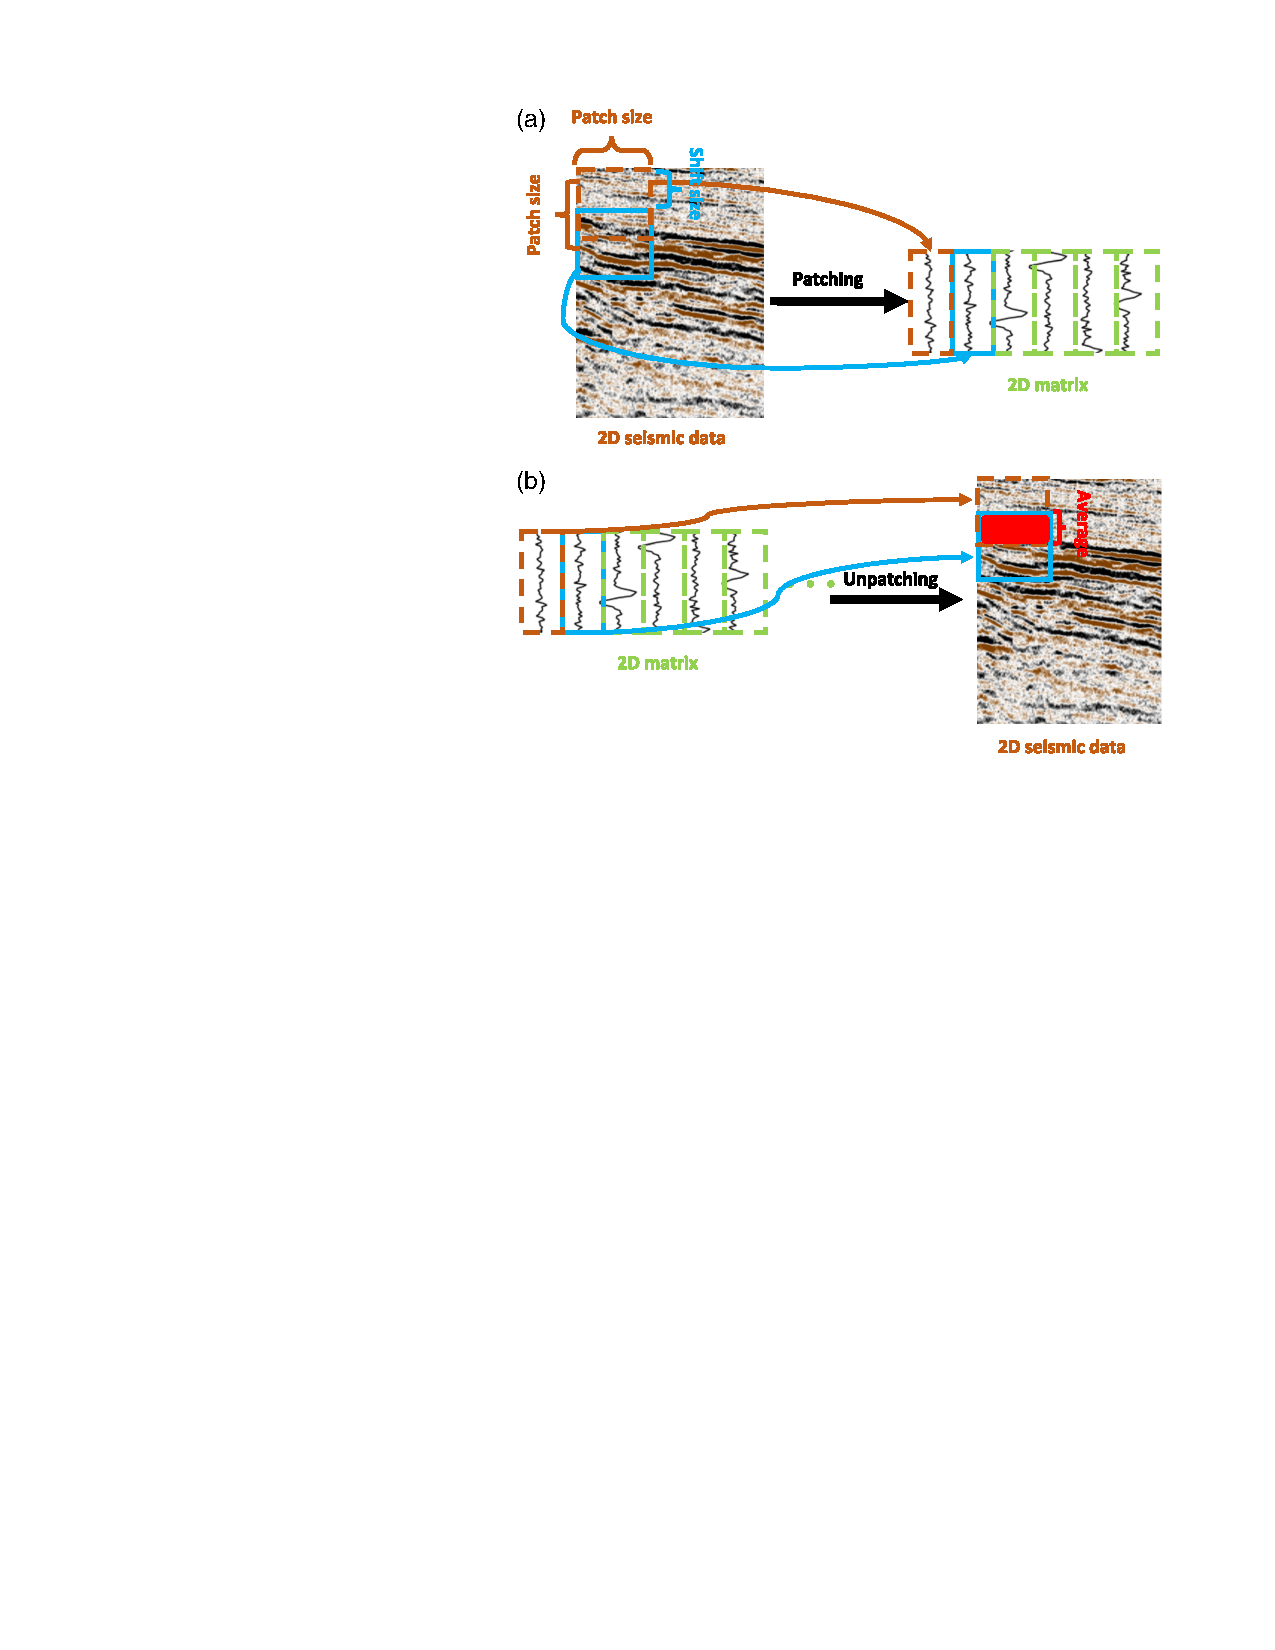
\includegraphics[width=0.8\textwidth]{Fig/demo}
	\caption{Demonstration of the structural flattening process in structure-oriented filtering.}
	\label{fig:demo}
\end{figure}


\begin{figure}[htb!]
	\centering
	\subfloat[]{\includegraphics[width=0.32\textwidth]{hyper/Fig/hyper}
    \label{fig:hyper}}
    \subfloat[]{\includegraphics[width=0.32\textwidth]{hyper/Fig/hyper-n}
    \label{fig:hyper-n}}
	\subfloat[]{\includegraphics[width=0.32\textwidth]{hyper/Fig/hyper-mf0}
    \label{fig:hyper-mf0}}\\
    \subfloat[]{\includegraphics[width=0.32\textwidth]{hyper/Fig/hyper-sosvmf0}
    \label{fig:hyper-sosvmf0}}
	\subfloat[]{\includegraphics[width=0.32\textwidth]{hyper/Fig/hyper-mf-n}
    \label{fig:hyper-mf-n}}
    \subfloat[]{\includegraphics[width=0.32\textwidth]{hyper/Fig/hyper-sosvmf-n}
    \label{fig:hyper-sosvmf-n}}\\
	\caption{\wen{Synthetic test for comparing different median filters. (a) Clean data. (b) Noisy data with strong erratic noise. (c) Denoised data using MF. (d) Denoised data using SOSVMF. (e) Removed noise using MF. (f) Removed noise using SOSVMF.}}
	\label{fig:hyper,hyper-n,hyper-mf0,hyper-sosvmf0,hyper-mf-n,hyper-sosvmf-n}
\end{figure}



\begin{figure}[htb!]
	\centering
	\subfloat[]{\includegraphics[width=0.38\textwidth]{Fig/l_dc}
    \label{fig:l_dc}}
    \subfloat[]{\includegraphics[width=0.38\textwidth]{Fig/l_dn}
    \label{fig:l_dn}}\\
	\caption{Synthetic example. (a) Clean data. (b) Noisy data (SNR=-1.25 dB). }
	\label{fig:l_dc,l_dn}
\end{figure}

\begin{figure}[htb!]
	\centering
	\subfloat[]{\includegraphics[width=0.38\textwidth]{Fig/l_curv}
    \label{fig:l_curv}}
    \subfloat[]{\includegraphics[width=0.38\textwidth]{Fig/l_sosvmf}
    \label{fig:l_sosvmf}}\\
	\subfloat[]{\includegraphics[width=0.38\textwidth]{Fig/l_curvi}
    \label{fig:l_curvi}}
    \subfloat[]{\includegraphics[width=0.38\textwidth]{Fig/l_sosvmfi}
    \label{fig:l_sosvmfi}}
	\caption{Synthetic example. (a) Denoised data using the curvelet method \wen{developed in \cite{candes20061} }(SNR=7.37 dB). (b) Denoised data using the single-step median filtering method \wen{developed in \cite{sosvmf} }(SNR=5.81 dB). (c) Denoised data using the iterative curvelet method \wen{developed in \cite{zhaoqiang2018} }(SNR=8.55 dB). (d) Denoised data using the proposed method (SNR=9.61 dB). }
	\label{fig:l_d}
\end{figure}

\begin{figure}[htb!]
	\centering
	\subfloat[]{\includegraphics[width=0.38\textwidth]{Fig/l_curv_n}
    \label{fig:l_curv_n}}
    \subfloat[]{\includegraphics[width=0.38\textwidth]{Fig/l_sosvmf_n}
    \label{fig:l_sosvmf_n}}\\
	\subfloat[]{\includegraphics[width=0.38\textwidth]{Fig/l_curvi_n}
    \label{fig:l_curvi_n}}
    \subfloat[]{\includegraphics[width=0.38\textwidth]{Fig/l_sosvmfi_n}
    \label{fig:l_sosvmfi_n}}
	\caption{Synthetic example. (a) Removed noise using the curvelet method. (b) Removed noise using the single-step median filtering method. (c) Removed noise using the iterative curvelet method. (d) Removed noise using the proposed method. \old{It is clear that the curvelet-related methods cause serious signal leakage while the median filtering-related methods do not cause obvious damages to signals. The proposed method removes more Gaussian-type noise than the single-step median filtering method. } }
	\label{fig:l_d_n}
\end{figure}

\begin{figure}[htb!]
	\centering
	\subfloat[]{\includegraphics[width=0.38\textwidth]{Fig/l_d_1}
    \label{fig:l_d_1}}
    \subfloat[]{\includegraphics[width=0.38\textwidth]{Fig/l_d_3}
    \label{fig:l_d_3}}\\
	\subfloat[]{\includegraphics[width=0.38\textwidth]{Fig/l_d_5}
    \label{fig:l_d_5}}
    \subfloat[]{\includegraphics[width=0.38\textwidth]{Fig/l_d_7}
    \label{fig:l_d_7}}\\
	\caption{Synthetic example. (a) Denoised data after 1 iteration. (b) Denoised data after 3 iterations.  (c) Denoised data after 5 iterations. (d) Denoised data after 7 iterations. }
	\label{fig:l_ds}
\end{figure}

\begin{figure}[htb!]
	\centering
	\subfloat[]{\includegraphics[width=0.38\textwidth]{Fig/l_n_1}
    \label{fig:l_n_1}}
    \subfloat[]{\includegraphics[width=0.38\textwidth]{Fig/l_n_3}
    \label{fig:l_n_3}}\\
	\subfloat[]{\includegraphics[width=0.38\textwidth]{Fig/l_n_5}
    \label{fig:l_n_5}}
    \subfloat[]{\includegraphics[width=0.38\textwidth]{Fig/l_n_7}
    \label{fig:l_n_7}}\\
	\caption{Synthetic example. (a) Removed noise after 1 iteration. (b) Removed noise after 3 iterations.  (c) Removed noise after 5 iterations. (d) Removed noise after 7 iterations. }
	\label{fig:l_ns}
\end{figure}

\begin{figure}[htb!]
	\centering
	\subfloat[]{\includegraphics[width=0.38\textwidth]{Fig/l_dip_dc}
    \label{fig:l_dip_dc}}
    \subfloat[]{\includegraphics[width=0.38\textwidth]{Fig/l_dip_dn}
    \label{fig:l_dip_dn}}\\
	\subfloat[]{\includegraphics[width=0.38\textwidth]{Fig/l_dip_1}
    \label{fig:l_dip_1}}
    \subfloat[]{\includegraphics[width=0.38\textwidth]{Fig/l_dip_3}
    \label{fig:l_dip_3}}\\
	\subfloat[]{\includegraphics[width=0.38\textwidth]{Fig/l_dip_5}
    \label{fig:l_dip_5}}
    \subfloat[]{\includegraphics[width=0.38\textwidth]{Fig/l_dip_7}
    \label{fig:l_dip_7}}\\
	\caption{\wen{Synthetic example. (a) Slope calculated from the clean data. (b) Slope calculated from the noisy data. (c) Calculated slope after 1 iteration. (d) Calculated slope after 3 iterations.  (e) Calculated slope after 5 iterations. (f) Calculated slope after 7 iterations.} }
	\label{fig:l_dips}
\end{figure}


\begin{figure}[htb!]
	\centering
	\includegraphics[width=0.8\textwidth]{Fig/l_snrs4}
	\caption{SNR variations during the iterative inversion.}
	\label{fig:l_snrs4}
\end{figure}


\begin{figure}[htb!]
	\centering
	\subfloat[]{\includegraphics[width=0.38\textwidth]{Fig/l_dd_1}
    \label{fig:l_dd_1}}
    \subfloat[]{\includegraphics[width=0.38\textwidth]{Fig/l_dd_3}
    \label{fig:l_dd_3}}\\
	\subfloat[]{\includegraphics[width=0.38\textwidth]{Fig/l_dd_5}
    \label{fig:l_dd_5}}
    \subfloat[]{\includegraphics[width=0.38\textwidth]{Fig/l_dd_7}
    \label{fig:l_dd_7}}\\
	\caption{Synthetic example (inversion without SOMF constraint). (a) Denoised data after 1 iteration. (b) Denoised data after 3 iterations.  (c) Denoised data after 5 iterations. (d) Denoised data after 7 iterations. }
	\label{fig:l_dds}
\end{figure}

\begin{figure}[htb!]
	\centering
	\subfloat[]{\includegraphics[width=0.38\textwidth]{Fig/l_nn_1}
    \label{fig:l_nn_1}}
    \subfloat[]{\includegraphics[width=0.38\textwidth]{Fig/l_nn_3}
    \label{fig:l_nn_3}}\\
	\subfloat[]{\includegraphics[width=0.38\textwidth]{Fig/l_nn_5}
    \label{fig:l_nn_5}}
    \subfloat[]{\includegraphics[width=0.38\textwidth]{Fig/l_nn_7}
    \label{fig:l_nn_7}}\\
	\caption{Synthetic example (inversion without SOMF constraint). (a) Removed noise after 1 iteration. (b) Removed noise after 3 iterations.  (c) Removed noise after 5 iterations. (d) Removed noise after 7 iterations. }
	\label{fig:l_nns}
\end{figure}


\begin{figure}[htb!]
	\centering
	\subfloat[]{\includegraphics[width=0.38\textwidth]{Fig/l_simi_curv}
    \label{fig:l_simi_curv}}
    \subfloat[]{\includegraphics[width=0.38\textwidth]{Fig/l_simi_sosvmf}
    \label{fig:l_simi_sosvmf}}\\
	\subfloat[]{\includegraphics[width=0.38\textwidth]{Fig/l_simi_curvi}
    \label{fig:l_simi_curvi}}
    \subfloat[]{\includegraphics[width=0.38\textwidth]{Fig/l_simi_sosvmfi}
    \label{fig:l_simi_sosvmfi}}
	\caption{Local similarity between clean data and denoised data. (a) Local similarity using the curvelet method. (b) Local similarity using the single-step median filtering method. (c) Local similarity using the iterative curvelet method. (d) Local similarity using the proposed method. }
	\label{fig:l_simi}
\end{figure}

\begin{figure}[htb!]
	\centering
	\subfloat[]{\includegraphics[width=0.38\textwidth]{Fig/l_simi2_curv}
    \label{fig:l_simi2_curv}}
    \subfloat[]{\includegraphics[width=0.38\textwidth]{Fig/l_simi2_sosvmf}
    \label{fig:l_simi2_sosvmf}}\\
	\subfloat[]{\includegraphics[width=0.38\textwidth]{Fig/l_simi2_curvi}
    \label{fig:l_simi2_curvi}}
    \subfloat[]{\includegraphics[width=0.38\textwidth]{Fig/l_simi2_sosvmfi}
    \label{fig:l_simi2_sosvmfi}}
	\caption{Local similarity between denoised data and removed noise. (a) Local similarity using the curvelet method. (b) Local similarity using the single-step median filtering method. (c) Local similarity using the iterative curvelet method. (d) Local similarity using the proposed method. }
	\label{fig:l_simi2}
\end{figure}



\begin{figure}[htb!]
	\centering
	\subfloat[]{\includegraphics[width=0.22\textwidth]{Fig/sigmas_dn1}
    \label{fig:sigmas_dn1}}
	\subfloat[]{\includegraphics[width=0.22\textwidth]{Fig/sigmas_dn2}
    \label{fig:sigmas_dn2}}
	\subfloat[]{\includegraphics[width=0.22\textwidth]{Fig/sigmas_dn3}
    \label{fig:sigmas_dn3}}
	\subfloat[]{\includegraphics[width=0.22\textwidth]{Fig/sigmas_dn4}
    \label{fig:sigmas_dn4}}\\
	\subfloat[]{\includegraphics[width=0.22\textwidth]{Fig/sigmas_d41}
    \label{fig:sigmas_d41}}
	\subfloat[]{\includegraphics[width=0.22\textwidth]{Fig/sigmas_d42}
    \label{fig:sigmas_d42}}
	\subfloat[]{\includegraphics[width=0.22\textwidth]{Fig/sigmas_d43}
    \label{fig:sigmas_d43}}
	\subfloat[]{\includegraphics[width=0.22\textwidth]{Fig/sigmas_d44}
    \label{fig:sigmas_d44}}\\ 
	\caption{\wen{Denoising test of different noise levels in terms of noise intensity. (a)-(d) Noisy data with the same erratic noise but with increasing random noise intensity. (e)-(h) \dlo{Removed noise}\wen{Denoised data} corresponding to (a)-(d), respectively. }}
	\label{fig:sigmas_d}
\end{figure}

\begin{figure}[htb!]
	\centering
	\subfloat[]{\includegraphics[width=0.22\textwidth]{Fig/dens_dn1}
    \label{fig:dens_dn1}}
	\subfloat[]{\includegraphics[width=0.22\textwidth]{Fig/dens_dn2}
    \label{fig:dens_dn2}}
	\subfloat[]{\includegraphics[width=0.22\textwidth]{Fig/dens_dn3}
    \label{fig:dens_dn3}}
	\subfloat[]{\includegraphics[width=0.22\textwidth]{Fig/dens_dn4}
    \label{fig:dens_dn4}}\\
	\subfloat[]{\includegraphics[width=0.22\textwidth]{Fig/dens_d41}
    \label{fig:dens_d41}}
	\subfloat[]{\includegraphics[width=0.22\textwidth]{Fig/dens_d42}
    \label{fig:dens_d42}}
	\subfloat[]{\includegraphics[width=0.22\textwidth]{Fig/dens_d43}
    \label{fig:dens_d43}}
	\subfloat[]{\includegraphics[width=0.22\textwidth]{Fig/dens_d44}
    \label{fig:dens_d44}}\\ 
	\caption{\wen{Denoising test of different noise levels in terms of density of erratic noise. (a)-(d) Noisy data with the same random noise but with increasing erratic noise density. (e)-(h) \dlo{Removed noise}\wen{Denoised data} corresponding to (a)-(d), respectively. }}
	\label{fig:dens_d}
\end{figure}





\begin{figure}[htb!]
	\centering
    \includegraphics[width=0.38\textwidth]{Fig/f_dn}
	\caption{\wen{First} field data example containing both Gaussian-type random noise and erratic noise.  }
	\label{fig:f_dn}
\end{figure}

\begin{figure}[htb!]
	\centering
	\subfloat[]{\includegraphics[width=0.38\textwidth]{Fig/f_curv}
    \label{fig:f_curv}}
    \subfloat[]{\includegraphics[width=0.38\textwidth]{Fig/f_sosvmf}
    \label{fig:f_sosvmf}}\\
	\subfloat[]{\includegraphics[width=0.38\textwidth]{Fig/f_curvi}
    \label{fig:f_curvi}}
    \subfloat[]{\includegraphics[width=0.38\textwidth]{Fig/f_sosvmfi}
    \label{fig:f_sosvmfi}}
	\caption{\wen{First} field data example. (a) Denoised data using the curvelet method. (b) Denoised data using the single-step median filtering method. (c) Denoised data using the iterative curvelet method. (d) Denoised data using the proposed method. }
	\label{fig:f_d}
\end{figure}

\begin{figure}[htb!]
	\centering
	\subfloat[]{\includegraphics[width=0.38\textwidth]{Fig/f_curv_n}
    \label{fig:f_curv_n}}
    \subfloat[]{\includegraphics[width=0.38\textwidth]{Fig/f_sosvmf_n}
    \label{fig:f_sosvmf_n}}\\
	\subfloat[]{\includegraphics[width=0.38\textwidth]{Fig/f_curvi_n}
    \label{fig:f_curvi_n}}
    \subfloat[]{\includegraphics[width=0.38\textwidth]{Fig/f_sosvmfi_n}
    \label{fig:f_sosvmfi_n}}
	\caption{\wen{First} field data example. (a) Removed noise using the curvelet method. (b) Removed noise using the single-step median filtering method. (c) Removed noise using the iterative curvelet method. (d) Removed noise using the proposed method. }
	\label{fig:f_d_n}
\end{figure}

\begin{figure}[htb!]
	\centering
	\subfloat[]{\includegraphics[width=0.38\textwidth]{Fig/f_d_1}
    \label{fig:f_d_1}}
    \subfloat[]{\includegraphics[width=0.38\textwidth]{Fig/f_d_3}
    \label{fig:f_d_3}}\\
	\subfloat[]{\includegraphics[width=0.38\textwidth]{Fig/f_d_5}
    \label{fig:f_d_5}}
    \subfloat[]{\includegraphics[width=0.38\textwidth]{Fig/f_d_7}
    \label{fig:f_d_7}}\\
	\caption{\wen{First} field data example. (a) Denoised data after 1 iteration. (b) Denoised data after 3 iterations.  (c) Denoised data after 5 iterations. (d) Denoised data after 7 iterations. }
	\label{fig:f_ds}
\end{figure}

\begin{figure}[htb!]
	\centering
	\subfloat[]{\includegraphics[width=0.38\textwidth]{Fig/f_n_1}
    \label{fig:f_n_1}}
    \subfloat[]{\includegraphics[width=0.38\textwidth]{Fig/f_n_3}
    \label{fig:f_n_3}}\\
	\subfloat[]{\includegraphics[width=0.38\textwidth]{Fig/f_n_5}
    \label{fig:f_n_5}}
    \subfloat[]{\includegraphics[width=0.38\textwidth]{Fig/f_n_7}
    \label{fig:f_n_7}}\\
	\caption{\wen{First} field data example. (a) Removed noise after 1 iteration. (b) Removed noise after 3 iterations.  (c) Removed noise after 5 iterations. (d) Removed noise after 7 iterations. }
	\label{fig:f_ns}
\end{figure}



\begin{figure}[htb!]
	\centering
	\subfloat[]{\includegraphics[width=0.38\textwidth]{Fig/f_simi2_curv}
    \label{fig:f_simi2_curv}}
    \subfloat[]{\includegraphics[width=0.38\textwidth]{Fig/f_simi2_sosvmf}
    \label{fig:f_simi2_sosvmf}}\\
	\subfloat[]{\includegraphics[width=0.38\textwidth]{Fig/f_simi2_curvi}
    \label{fig:f_simi2_curvi}}
    \subfloat[]{\includegraphics[width=0.38\textwidth]{Fig/f_simi2_sosvmfi}
    \label{fig:f_simi2_sosvmfi}}
	\caption{Local similarity between denoised data and removed noise for the \wen{first} field data example. (a) Local similarity using the curvelet method. (b) Local similarity using the single-step median filtering method. (c) Local similarity using the iterative curvelet method. (d) Local similarity using the proposed method. }
	\label{fig:f_simi2}
\end{figure}


\begin{figure}[htb!]
	\centering
	\subfloat[]{\includegraphics[width=0.38\textwidth]{Fig/f2_dn}
    \label{fig:f2_dn}}\\
	\subfloat[]{\includegraphics[width=0.38\textwidth]{Fig/f2_curv}
    \label{fig:f2_curv}}
    \subfloat[]{\includegraphics[width=0.38\textwidth]{Fig/f2_sosvmf}
    \label{fig:f2_sosvmf}}\\
	\subfloat[]{\includegraphics[width=0.38\textwidth]{Fig/f2_curvi}
    \label{fig:f2_curvi}}
    \subfloat[]{\includegraphics[width=0.38\textwidth]{Fig/f2_sosvmfi}
    \label{fig:f2_sosvmfi}}
	\caption{\wen{Second field data example. (a) Field data containing both Gaussian-type random noise and erratic noise. (b) Denoised data using the curvelet method. (c) Denoised data using the single-step median filtering method. (d) Denoised data using the iterative curvelet method. (e) Denoised data using the proposed method. \new{The two pink arrows indicate potential residual spikes.}} }
	\label{fig:f2_d}
\end{figure}


\begin{figure}[htb!]
	\centering
	\subfloat[]{\includegraphics[width=0.38\textwidth]{Fig/f2_curv_n}
    \label{fig:f2_curv_n}}
    \subfloat[]{\includegraphics[width=0.38\textwidth]{Fig/f2_sosvmf_n}
    \label{fig:f2_sosvmf_n}}\\
	\subfloat[]{\includegraphics[width=0.38\textwidth]{Fig/f2_curvi_n}
    \label{fig:f2_curvi_n}}
    \subfloat[]{\includegraphics[width=0.38\textwidth]{Fig/f2_sosvmfi_n}
    \label{fig:f2_sosvmfi_n}}
	\caption{\wen{Second field data example. (a) Removed noise using the curvelet method. (b) Removed noise using the single-step median filtering method. (c) Removed noise using the iterative curvelet method. (d) Removed noise using the proposed method.} }
	\label{fig:f2_d_n}
\end{figure}

}

\newpage
\listoffigures
\newpage


